\documentclass{article}
\usepackage{booktabs}
\usepackage{caption} % Include the caption package
\captionsetup{justification=raggedright,singlelinecheck=false}
\usepackage{graphicx}
\usepackage{pgf}


\begin{document}


\textbf{Here we se the growth rates in the different scenarios}

 
\begin{figure}[htbp]
\centering
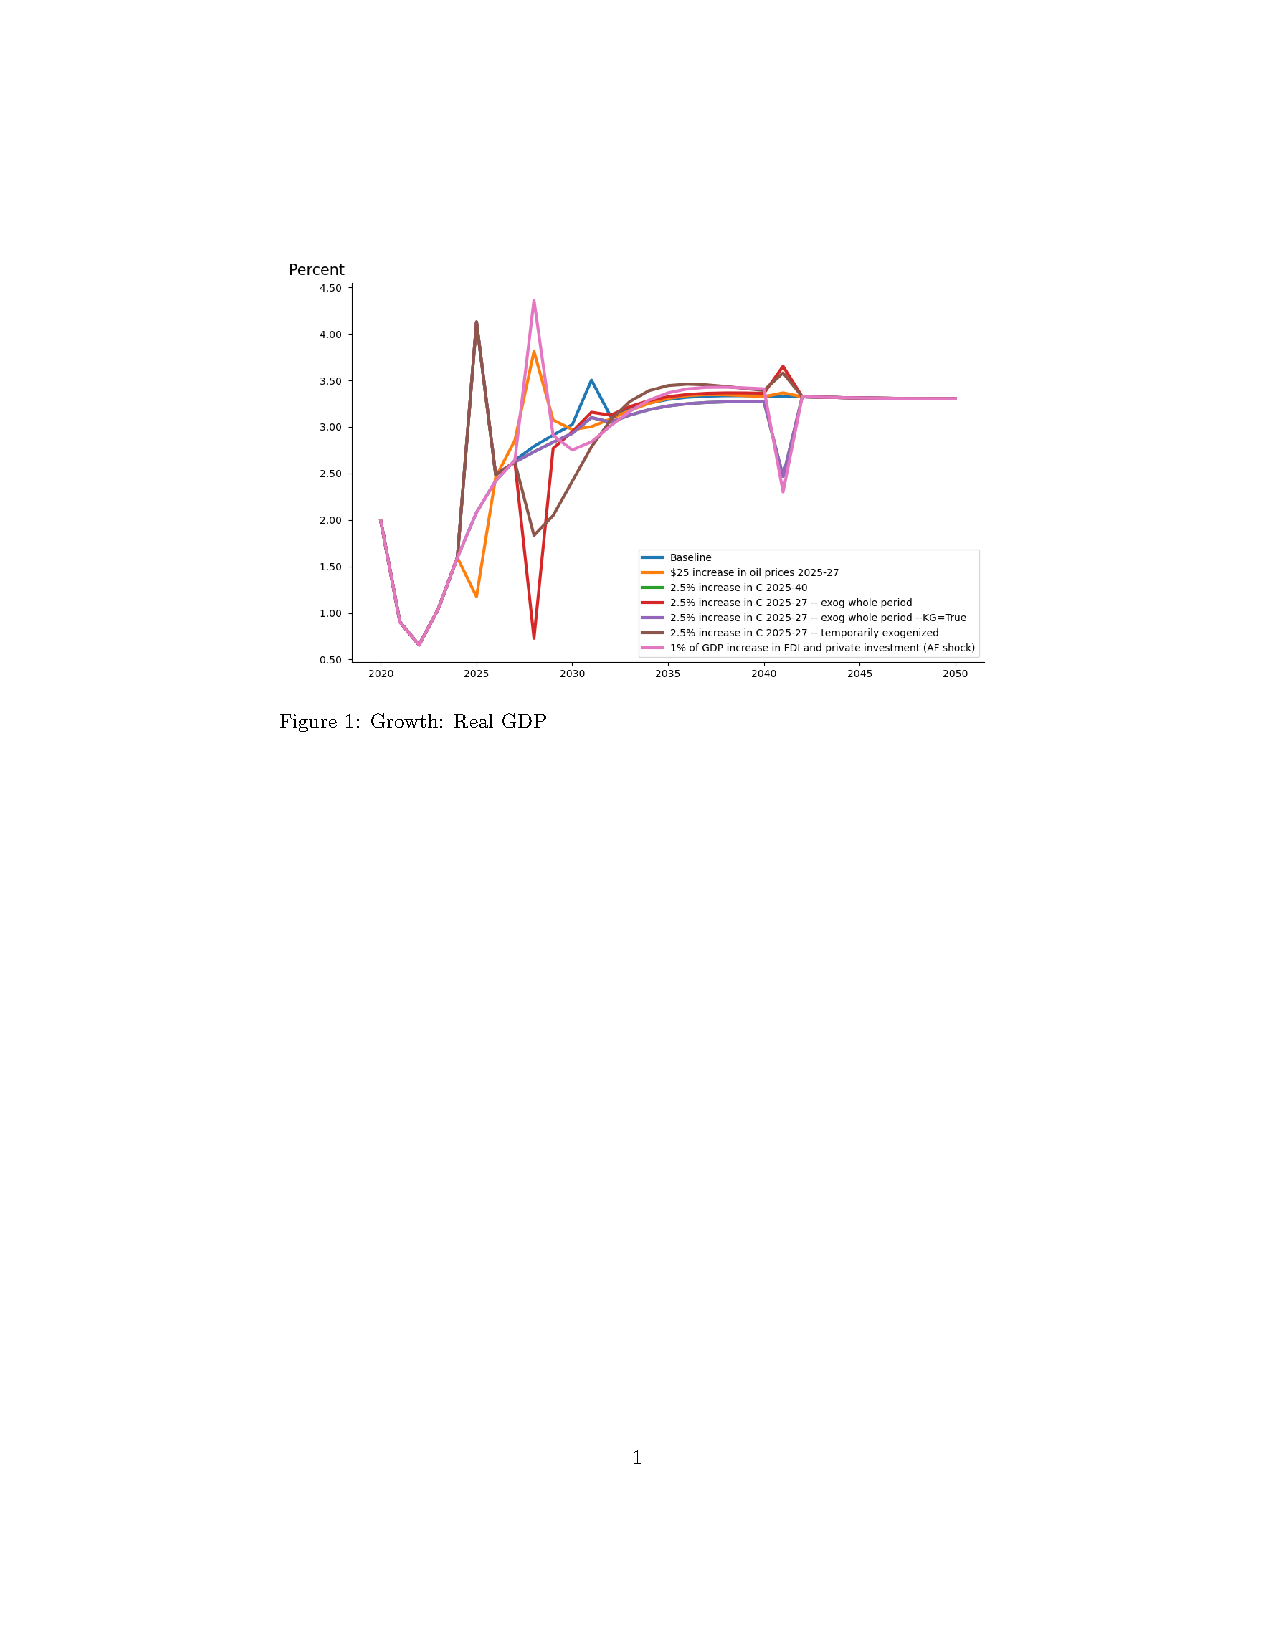
\includegraphics[width=\textwidth]{"../My_first_plot/My_first_plot.png"}
\caption{}
\end{figure} 

\textbf{Then a table}

\begin{table}[ht]
\caption{GDP components}
\begin{tabular}{lrrrrr}
\toprule
 & Real GDP & HH. Cons Real & Investment real & Exports real & Imports real \\
\midrule
&\multicolumn{5}{c}{{--- Percent growth ---}}\\
2022 & 0.66 & 0.80 & 0.70 & 4.71 & 3.00 \\
2023 & 1.04 & 1.09 & 0.63 & 4.66 & 2.86 \\
2024 & 1.60 & 1.60 & 0.79 & 4.53 & 2.99 \\
2025 & 2.08 & 2.03 & 1.10 & 4.37 & 3.10 \\
2026 & 2.42 & 2.32 & 1.46 & 4.20 & 3.10 \\
2027 & 2.64 & 2.48 & 1.82 & 4.04 & 3.02 \\
\bottomrule
\end{tabular}
\caption*{Source: World bank }
\end{table}

\end{document}
        